% Standalone: Actual KG path — Varroa Destructor → Polyface
% All node names, edge keywords, and descriptions are real graph data from
%   data/working_dir/agriculture/graph_chunk_entity_relation.graphml
% Path found via nx.shortest_path (3 hops, 4 nodes)
% Compile: pdflatex fig_varroa_path.tex
\documentclass[tikz,border=14pt]{standalone}
\usepackage{tikz}
\usetikzlibrary{arrows.meta, positioning, backgrounds, fit, shadows, shapes.misc}
\usepackage[T1]{fontenc}

% ── Colour palette ────────────────────────────────────────────────────────────
\definecolor{anchorblue}{RGB}{37,99,235}
\definecolor{bridgeorange}{RGB}{234,88,12}
\definecolor{nbgray}{RGB}{120,130,145}
\definecolor{edgepath}{RGB}{234,88,12}
\definecolor{edgenb}{RGB}{180,190,200}
\definecolor{nodebg}{RGB}{255,255,255}

\begin{document}
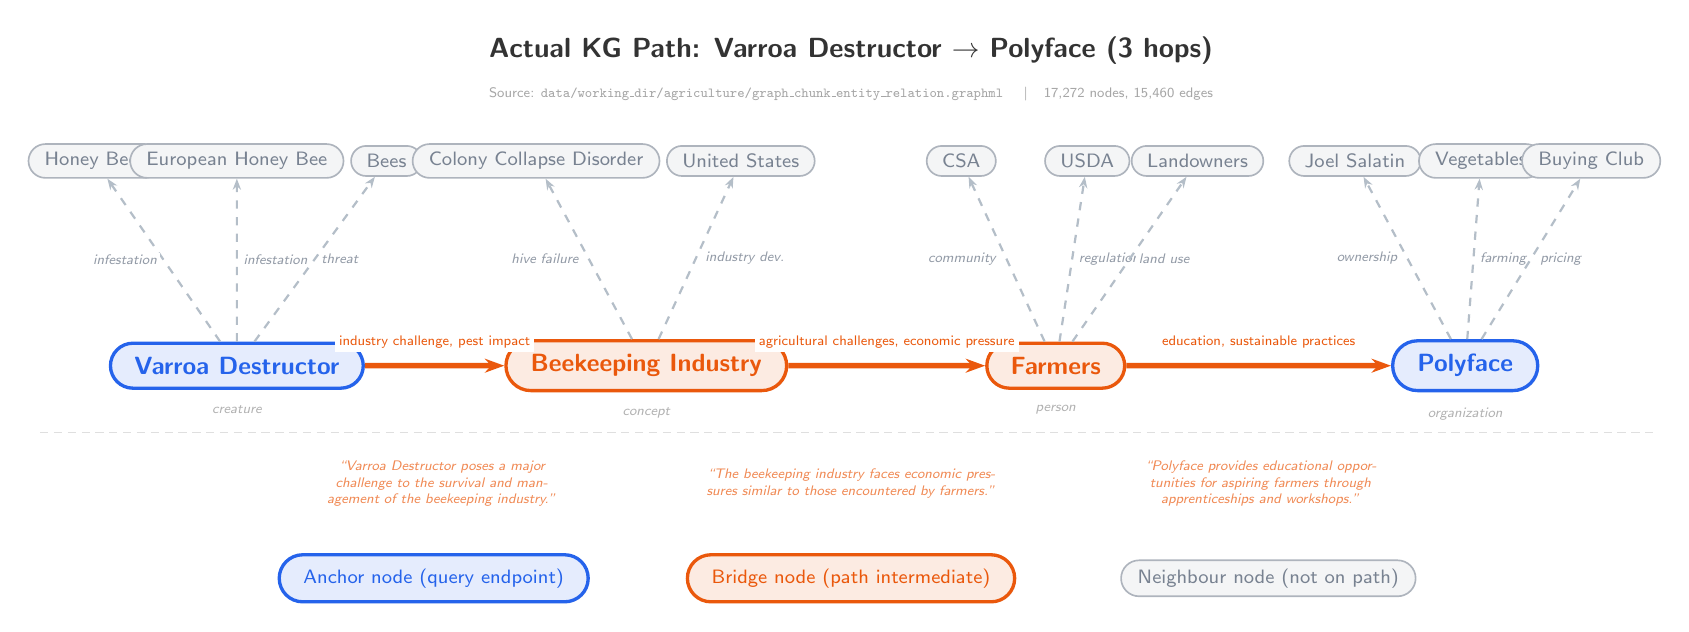
\begin{tikzpicture}[
  % ── node styles ─────────────────────────────────────────────────────────────
  anode/.style = {
    rounded rectangle, draw=anchorblue, fill=anchorblue!12,
    line width=1.2pt, font=\small\bfseries\sffamily, text=anchorblue,
    inner xsep=8pt, inner ysep=5pt,
    drop shadow={shadow xshift=0.5pt, shadow yshift=-0.5pt, opacity=0.15}
  },
  bridge/.style = {
    rounded rectangle, draw=bridgeorange, fill=bridgeorange!12,
    line width=1.2pt, font=\small\bfseries\sffamily, text=bridgeorange,
    inner xsep=8pt, inner ysep=5pt,
    drop shadow={shadow xshift=0.5pt, shadow yshift=-0.5pt, opacity=0.15}
  },
  nbnode/.style = {
    rounded rectangle, draw=nbgray!60, fill=nbgray!8,
    line width=0.6pt, font=\scriptsize\sffamily, text=nbgray,
    inner xsep=5pt, inner ysep=3pt
  },
  % ── edge styles ─────────────────────────────────────────────────────────────
  pathline/.style = {
    draw=edgepath, line width=2pt,
    -{Stealth[length=7pt, width=5pt]},
  },
  nbline/.style = {
    draw=edgenb, line width=0.8pt, dashed,
    -{Stealth[length=4pt, width=3pt]},
  },
  % ── label styles ────────────────────────────────────────────────────────────
  edgelabel/.style = {
    font=\tiny\sffamily, text=edgepath, fill=white,
    inner sep=1.5pt
  },
  nblabel/.style = {
    font=\tiny\sffamily, text=nbgray!80, fill=white,
    inner sep=1pt
  },
  typetag/.style = {
    font=\tiny\sffamily\itshape, text=gray!60
  },
]

%% ═══════════════════════════════════════════════════════════════════════════
%%  MAIN PATH NODES  (horizontal, y=0)
%% ═══════════════════════════════════════════════════════════════════════════

\node[anode] (vd)  at (0,   0) {Varroa Destructor};
\node[bridge] (bi)  at (5.2, 0) {Beekeeping Industry};
\node[bridge] (fa)  at (10.4,0) {Farmers};
\node[anode] (pf)  at (15.6,0) {Polyface};

% entity type tags below each main node
\node[typetag, below=2pt of vd] {creature};
\node[typetag, below=2pt of bi] {concept};
\node[typetag, below=2pt of fa] {person};
\node[typetag, below=2pt of pf] {organization};

%% ═══════════════════════════════════════════════════════════════════════════
%%  PATH EDGES  (with real keywords)
%% ═══════════════════════════════════════════════════════════════════════════

\draw[pathline] (vd) -- node[edgelabel, above=4pt]
  {industry challenge, pest impact} (bi);

\draw[pathline] (bi) -- node[edgelabel, above=4pt]
  {agricultural challenges, economic pressure} (fa);

\draw[pathline] (fa) -- node[edgelabel, above=4pt]
  {education, sustainable practices} (pf);

%% ═══════════════════════════════════════════════════════════════════════════
%%  NEIGHBOUR NODES  (real adjacent nodes from the graph)
%% ═══════════════════════════════════════════════════════════════════════════

%% Varroa Destructor neighbours (above)
\node[nbnode] (nb_vd1) at (-1.8,  2.6) {Honey Bees};
\node[nbnode] (nb_vd2) at ( 0,    2.6) {European Honey Bee};
\node[nbnode] (nb_vd3) at ( 1.9,  2.6) {Bees};

\draw[nbline] (vd) -- node[nblabel, left=1pt] {\textit{infestation}} (nb_vd1);
\draw[nbline] (vd) -- node[nblabel, right=1pt] {\textit{infestation}} (nb_vd2);
\draw[nbline] (vd) -- node[nblabel, right=1pt] {\textit{threat}} (nb_vd3);

%% Beekeeping Industry neighbours (above)
\node[nbnode] (nb_bi1) at (3.8,  2.6) {Colony Collapse Disorder};
\node[nbnode] (nb_bi2) at (6.4,  2.6) {United States};

\draw[nbline] (bi) -- node[nblabel, left=2pt] {\textit{hive failure}} (nb_bi1);
\draw[nbline] (bi) -- node[nblabel, right=2pt] {\textit{industry dev.}} (nb_bi2);

%% Farmers neighbours (above)
\node[nbnode] (nb_fa1) at (9.2,  2.6) {CSA};
\node[nbnode] (nb_fa2) at (10.8, 2.6) {USDA};
\node[nbnode] (nb_fa3) at (12.2, 2.6) {Landowners};

\draw[nbline] (fa) -- node[nblabel, left=2pt] {\textit{community}} (nb_fa1);
\draw[nbline] (fa) -- node[nblabel, right=1pt] {\textit{regulation}} (nb_fa2);
\draw[nbline] (fa) -- node[nblabel, right=2pt] {\textit{land use}} (nb_fa3);

%% Polyface neighbours (above)
\node[nbnode] (nb_pf1) at (14.2, 2.6) {Joel Salatin};
\node[nbnode] (nb_pf2) at (15.8, 2.6) {Vegetables};
\node[nbnode] (nb_pf3) at (17.2, 2.6) {Buying Club};

\draw[nbline] (pf) -- node[nblabel, left=2pt] {\textit{ownership}} (nb_pf1);
\draw[nbline] (pf) -- node[nblabel, right=1pt] {\textit{farming}} (nb_pf2);
\draw[nbline] (pf) -- node[nblabel, right=2pt] {\textit{pricing}} (nb_pf3);

%% ═══════════════════════════════════════════════════════════════════════════
%%  EDGE DESCRIPTIONS  (real, below the path)
%% ═══════════════════════════════════════════════════════════════════════════

\node[font=\tiny\sffamily, text=edgepath!70, text width=3.5cm, align=center]
  at (2.6, -1.5)
  {\textit{``Varroa Destructor poses a major challenge to the survival and
   management of the beekeeping industry.''}};

\node[font=\tiny\sffamily, text=edgepath!70, text width=3.8cm, align=center]
  at (7.8, -1.5)
  {\textit{``The beekeeping industry faces economic pressures similar to those
   encountered by farmers.''}};

\node[font=\tiny\sffamily, text=edgepath!70, text width=3.5cm, align=center]
  at (13.0, -1.5)
  {\textit{``Polyface provides educational opportunities for aspiring farmers
   through apprenticeships and workshops.''}};

% Dashed line separating description from main graph
\draw[gray!25, densely dashed] (-2.5, -0.85) -- (18, -0.85);

%% ═══════════════════════════════════════════════════════════════════════════
%%  TITLE + LEGEND
%% ═══════════════════════════════════════════════════════════════════════════

\node[font=\normalsize\bfseries\sffamily, text=black!80]
  at (7.8, 4.0)
  {Actual KG Path: Varroa Destructor $\to$ Polyface (3 hops)};

\node[font=\tiny\sffamily, text=gray!70]
  at (7.8, 3.45)
  {Source: \texttt{data/working\_dir/agriculture/graph\_chunk\_entity\_relation.graphml}
   \quad $|$\quad 17,272 nodes, 15,460 edges};

% Legend
\node[anode, font=\scriptsize\sffamily]
  at (2.5, -2.7) {Anchor node (query endpoint)};

\node[bridge, font=\scriptsize\sffamily]
  at (7.8, -2.7) {Bridge node (path intermediate)};

\node[nbnode]
  at (13.1, -2.7) {Neighbour node (not on path)};

\end{tikzpicture}
\end{document}
